%\documentclass[handout]{beamer}
\documentclass{beamer}

\mode<presentation>
{
\usetheme{default}
\usefonttheme[onlymath]{serif}
%\usetheme{Singapore}
%\usetheme{Warsaw}
%\usetheme{Malmoe}
% \useinnertheme{circles}
% \useoutertheme{infolines}
% \useinnertheme{rounded}

\setbeamercovered{transparent=5}
}

\usepackage[english]{babel}
\usepackage[latin1]{inputenc}
\usepackage{textpos,alltt,listings,multirow,ulem,siunitx}
\newcommand\hmmax{0}
\newcommand\bmmax{0}
\usepackage{bm}

% font definitions, try \usepackage{ae} instead of the following
% three lines if you don't like this look
\usepackage{mathptmx}
\usepackage[scaled=.90]{helvet}
%\usepackage{courier}
\usepackage[T1]{fontenc}
\usepackage{tikz}
\usetikzlibrary[shapes,shapes.arrows,arrows,shapes.misc,fit,positioning]

% \usepackage{pgfpages}
% \pgfpagesuselayout{4 on 1}[a4paper,landscape,border shrink=5mm]

\usepackage{slashbox,multirow,listings,booktabs}
\usepackage{xspace}
\makeatletter
\DeclareRobustCommand\onedot{\futurelet\@let@token\@onedot}
\def\@onedot{\ifx\@let@token.\else.\null\fi\xspace}
\def\eg{{e.g}\onedot} \def\Eg{{E.g}\onedot}
\def\ie{{i.e}\onedot} \def\Ie{{I.e}\onedot}
\def\cf{{c.f}\onedot} \def\Cf{{C.f}\onedot}
\def\etc{{etc}\onedot}
\def\vs{{vs}\onedot}
\def\wrt{w.r.t\onedot}
\def\dof{d.o.f\onedot}
\def\etal{{et al}\onedot}
\makeatother

\usepackage{tikz}
\usetikzlibrary[shapes,shapes.arrows,arrows,shapes.misc,fit,positioning]

\usepackage{siunitx}
\DeclareSIUnit\year{a}
\DeclareSIUnit\byte{B}
\sisetup{retain-unity-mantissa = false}

\usepackage{fancyvrb}
\usepackage{minted}
\newminted{c}{gobble=2}
\newminted{python}{gobble=2}
%\newmint[cverb]{c}{} 
\newcommand\cverb[1][]{\SaveVerb[%
    aftersave={\textnormal{\UseVerb[#1]{vsave}}}]{vsave}}
\newcommand\cfunc[1][]{\SaveVerb[%
    aftersave={\textnormal{\UseVerb[#1]{vsave}\texttt{()}}}]{vsave}}
\newcommand\pyverb[1][]{\SaveVerb[%
    aftersave={\textnormal{\UseVerb[#1]{vsave}}}]{vsave}}
\def\asm#1{{\tt #1}}
\def\code#1{{\tt #1}}
\def\shell#1{{\tt \$ #1}}

\newcommand\email[1]{{\href{mailto:#1}{\nolinkurl{#1}}}}

\newcommand{\II}{\mathcal{I}}
\newcommand{\C}{\mathbb{C}}
\newcommand{\D}{\mathcal{D}}
\newcommand{\EE}{\mathcal{E}}
\newcommand{\F}{\mathcal{F}}
\newcommand{\I}{\mathcal{I}}
\newcommand{\N}{\mathcal{N}}
\newcommand{\PP}{\mathcal{P}}
\newcommand\Ppc{\ensuremath{\mathsf P}}
\newcommand{\bigO}{\ensuremath{\mathcal{O}}}
\newcommand{\R}{\mathbb{R}}
\newcommand{\Rz}{\mathcal{R}}
\newcommand{\QQ}{\mathcal Q}
\newcommand{\VV}{\mathcal V}
\newcommand{\ASM}{\mathrm{ASM}}
\newcommand{\RASM}{\mathrm{RASM}}

\newcommand{\kb}{\tt}
\newcommand{\Pk}[1]{\ensuremath{P_{#1}}}
\newcommand{\Qk}[1]{\ensuremath{Q_{#1}}}
\newcommand{\Pkdisc}[1]{\ensuremath{P_{#1}^{\text{disc}}}}
\newcommand{\Qkdisc}[1]{\ensuremath{Q_{#1}^{\text{disc}}}}
\newcommand{\blue}{\textcolor{blue}}
\newcommand{\green}{\textcolor{green!70!black}}
\newcommand{\red}{\textcolor{red}}
\newcommand{\brown}{\textcolor{brown}}
\newcommand{\cyan}{\textcolor{cyan}}
\newcommand{\magenta}{\textcolor{magenta}}
\newcommand{\yellow}{\textcolor{yellow}}
\newcommand{\mini}{\mathop{\rm minimize}}
\newcommand{\st}{\mbox{subject to }}
\newcommand{\lap}{\Delta}
\newcommand{\grad}{\nabla}
\newcommand\mtab{\hspace{\stretch{1}}}
\newcommand\ud{\,\mathrm{d}}
\newcommand\bslash{{$\backslash$}}
\newcommand\half{{\frac 1 2}}
\newcommand{\abs}[1]{\left\lvert #1 \right\rvert}
\newcommand{\bigabs}[1]{\big\lvert #1 \big\rvert}
\newcommand{\norm}[1]{\left\lVert #1 \right\rVert}
\newcommand\oneitem[1]{\begin{itemize} \item #1 \end{itemize}}
\newcommand\pfrak{{\mathfrak p}}
\newcommand\nfrak{{\mathfrak n}}
\newcommand\ff{\bm f}
\newcommand\mm{\bm m}
\newcommand\nn{\bm n}
\newcommand\uu{\bm u}
\newcommand\vv{\bm v}
\newcommand\ww{\bm w}
\newcommand\DD{D}
\newcommand{\tcolon}{\!:\!}
\DeclareMathOperator{\sgn}{sgn}
\DeclareMathOperator{\card}{card}
\DeclareMathOperator{\trace}{tr}
\DeclareMathOperator{\erf}{erf}
\DeclareMathOperator{\sspan}{span}
\renewcommand{\bar}{\overline}
% \DeclareMathOperator{\divergence}{div}
% \renewcommand\div\divergence
\renewcommand{\div}{{\nabla \cdot}}
\newcommand\spliceop{\leftrightsquigarrow}
\newcommand\splice[5]{{#1} \overset{#5}{\underset{#3,#4}{\leftrightsquigarrow}} {#2}}
\newcommand{\ip}[2]{{\left\langle #1, #2 \right\rangle}}
\newcommand{\Linfty}{{L^\infty}}

% Dimensionless numbers
\newcommand{\Peclet}{{\mathrm{Pe}}}
\newcommand{\Reynolds}{{\mathrm{Re}}}
\newcommand{\Rayleigh}{{\mathrm{Ra}}}
\newcommand{\Mach}{{\mathrm{Ma}}}
\newcommand{\Prandtl}{{\mathrm{Pr}}}
\newcommand{\Grashof}{{\mathrm{Gr}}}

\newcommand{\PETSc}{{PETSc}}
\newcommand{\Dohp}{{Dohp}}
\newcommand\libmesh{\texttt{libMesh}}
\newcommand\dealii{\texttt{Deal.II}}
\newcommand\MatMult{\cverb|MatMult|}
\newcommand\MatSolve{\cverb|MatSolve|}
\newcommand{\secref}[1]{{Section~\ref{#1}}}
\newcommand{\chapref}[1]{{Chapter~\ref{#1}}}
\newcommand{\figref}[1]{{Figure~\ref{#1}}}
\newcommand{\tabref}[1]{{Table~\ref{#1}}}
\newcommand\AIJ{{\cverb|AIJ|}}
\newcommand\AIJInode{\cverb|AIJ|/\cverb|Inode|}
\newcommand\BAIJ[1][]{\ifthenelse{\equal{#1}{}}{\cverb|BAIJ|}{\ensuremath{\cverb|BAIJ|(#1)}}}
\newcommand\SBAIJ[1][]{\ifthenelse{\equal{#1}{}}{\cverb|SBAIJ|}{\ensuremath{\cverb|SBAIJ|(#1)}}}
\newcommand\todo[1]{{\color{red}\bf [TODO: #1]}}
\newcommand\tf[1]{\hat{#1}}     % test functions


\title{Verifying correctness of PDE solvers using SymPy}

\author{Jed Brown}


% - Use the \inst command only if there are several affiliations.
% - Keep it simple, no one is interested in your street address.
\institute[ANL]
{
  {Argonne National Laboratory} / {ETH Z\"urich}
}

\date{2011-07-14}

% This is only inserted into the PDF information catalog. Can be left
% out.
\subject{Talks}


% If you have a file called "university-logo-filename.xxx", where xxx
% is a graphic format that can be processed by latex or pdflatex,
% resp., then you can add a logo as follows:

% \pgfdeclareimage[height=0.5cm]{university-logo}{university-logo-filename}
% \logo{\pgfuseimage{university-logo}}



% Delete this, if you do not want the table of contents to pop up at
% the beginning of each subsection:
% \AtBeginSubsection[]
% {
% \begin{frame}<beamer>
% \frametitle{Outline}
% \tableofcontents[currentsection,currentsubsection]
% \end{frame}
% }

% If you wish to uncover everything in a step-wise fashion, uncomment
% the following command:

%\beamerdefaultoverlayspecification{<+->}

\begin{document}
\lstset{language=C}
\normalem

\begin{frame}
\titlepage
\end{frame}

\begin{frame}[fragile,shrink=5]{Symbolic form of large-deformation elasticity}
  Find displacement vector $\uu$ such that:
  \begin{equation*}
    \int_\Omega \nabla \vv \tcolon \Pi = 0,\quad \forall \vv
  \end{equation*}
  where
  \begin{align*}
    F   & = I - \nabla \uu                &  & \text{Deformation gradient}  \\
    E   & = (F^T F - I)/2                 &  & \text{Green-Lagrange tensor} \\
    S   & = \lambda (\trace E) I + 2\mu E &  & \text{Second Piola-Kirchoff tensor} \\
    \Pi & = F \cdot S                     &  & \text{First Piola-Kirchoff tensor}
  \end{align*}
\begin{pythoncode}
  def weak_form(u, du, v, dv):
    I = eye(3)                      # Identity tensor
    F = I - du                      # Deformation gradient
    E = (F.T*F - I)/2               # Green-Lagrange tensor
    S = lmbda*E.trace()*I + 2*mu*E  # Second Piola-Kirchoff tensor
    Pi = F * S                      # First Piola-Kirchoff tensor
    return dv.dot(Pi)
\end{pythoncode}
\end{frame}

\begin{frame}[fragile]{Manufactured solution}
  \begin{itemize}
  \item Choose a solution $\uu_{\text{exact}}$ with rich derivatives
  \begin{pythoncode}
  def solution(x,y,z, a,b,c):
    return Matrix([cos(x) * exp(y) * z + sin(z),
                   sin(x) * tanh(y) + x * cosh(z),
                   exp(x) * sinh(y) + y * log(1+z**2)])
  \end{pythoncode}
  \item Apply strong-form nonlinear differential operator symbolically
    to define
    \[ f(x,y,z) = \nabla\cdot \Pi(\nabla \uu_{\text{exact}}) \]
  \item Solve finite element problem for $\uu_h$
    \begin{equation*}
      \int_\Omega \nabla \vv \tcolon \Pi(\nabla \uu_h) = \int v\cdot f(x,y,z),\quad \forall \vv
    \end{equation*}
  \item Compute norms of $\uu_h - \uu_{\text{exact}}$.
  \end{itemize}
\end{frame}

\begin{frame}{Manufactured solution}
  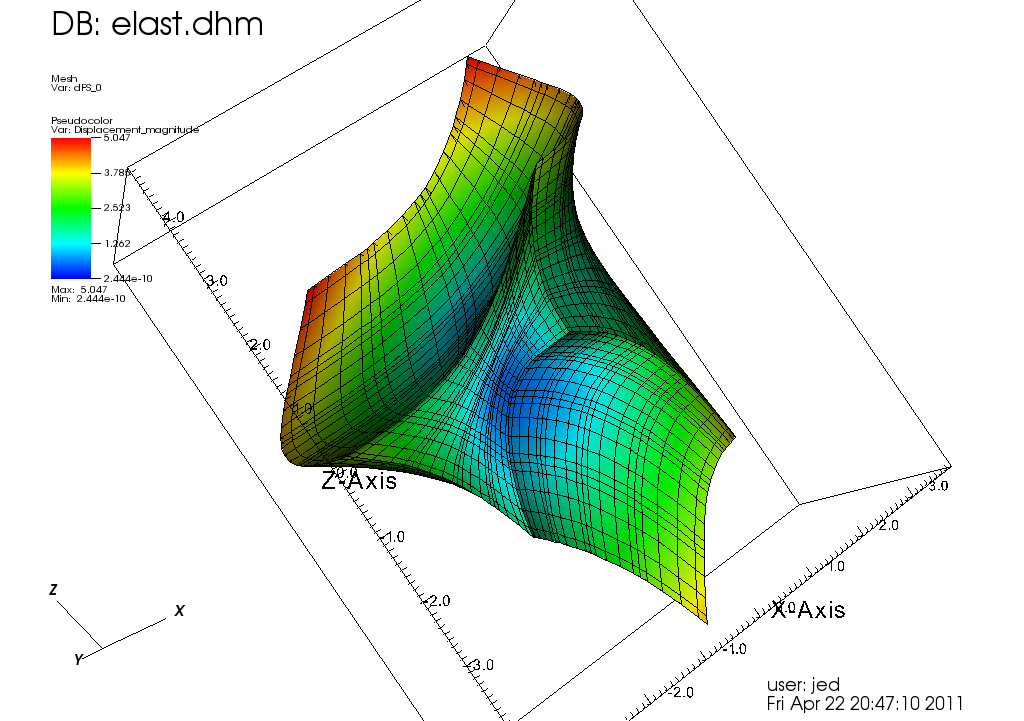
\includegraphics[width=\textwidth]{figures/elast-b4q5} \\
\end{frame}

\begin{frame}[shrink=30]{Convergence rates}
  \begin{tabular}{lrr rr rr rr rr}
    \toprule
    & & & \multicolumn{2}{c}{$\norm{\uu_h - \uu}_2$} & \multicolumn{2}{c}{$\norm{\uu_h - \uu}_\infty$}
    & \multicolumn{2}{c}{$\norm{\nabla\uu_h - \nabla\uu}_2$} & \multicolumn{2}{c}{$\norm{\nabla\uu_h - \nabla\uu}_\infty$} \\
    \cmidrule(r){4-5} \cmidrule(lr){6-7} \cmidrule(lr){8-9} \cmidrule(l){10-11}
    \multicolumn{2}{c}{Mesh} & \# Nodes & Error & \bigO & Error & \bigO & Error & \bigO & Error & \bigO \\
    \midrule % output below is generated with verif.py in this directory
$Q_1$ & $1^3$ & 8 & 1.79e+00 & --- & 6.50e-01 & --- & 3.70e+00 & --- & 1.08e+00 & --- \\
$Q_1$ & $2^3$ & 27 & 5.49e-01 & 1.71 & 3.40e-01 & 0.93 & 1.61e+00 & 1.20 & 6.92e-01 & 0.64 \\
$Q_1$ & $4^3$ & 125 & 1.53e-01 & 1.84 & 1.26e-01 & 1.43 & 8.01e-01 & 1.01 & 4.51e-01 & 0.62 \\
$Q_1$ & $8^3$ & 729 & 3.94e-02 & 1.96 & 3.73e-02 & 1.76 & 3.98e-01 & 1.01 & 2.81e-01 & 0.68 \\
$Q_1$ & $16^3$ & 4913 & 9.95e-03 & 1.99 & 1.01e-02 & 1.88 & 1.98e-01 & 1.01 & 1.57e-01 & 0.84 \\
$Q_1$ & $32^3$ & 35937 & 2.49e-03 & 2.00 & 2.61e-03 & 1.95 & 9.92e-02 & 1.00 & 8.32e-02 & 0.92\\
% \midrule
% $Q_2$ & $1^3$ & 27 & 2.44e-01 & --- & 1.82e-01 & --- & 9.48e-01 & --- & 4.60e-01 & --- \\
% $Q_2$ & $2^3$ & 125 & 3.71e-02 & 2.72 & 4.47e-02 & 2.03 & 2.86e-01 & 1.73 & 1.54e-01 & 1.58 \\
% $Q_2$ & $4^3$ & 729 & 4.48e-03 & 3.05 & 6.23e-03 & 2.84 & 6.94e-02 & 2.04 & 4.34e-02 & 1.83 \\
% $Q_2$ & $8^3$ & 4913 & 5.60e-04 & 3.00 & 9.31e-04 & 2.74 & 1.74e-02 & 2.00 & 1.29e-02 & 1.75 \\
% $Q_2$ & $16^3$ & 35937 & 7.01e-05 & 3.00 & 1.23e-04 & 2.92 & 4.34e-03 & 2.00 & 3.52e-03 & 1.87\\
\midrule
$Q_3$ & $1^3$ & 64 & 4.14e-02 & --- & 2.71e-02 & --- & 2.90e-01 & --- & 1.63e-01 & --- \\
$Q_3$ & $2^3$ & 343 & 2.06e-03 & 4.33 & 2.06e-03 & 3.72 & 2.39e-02 & 3.60 & 1.14e-02 & 3.84 \\
$Q_3$ & $4^3$ & 2197 & 1.81e-04 & 3.51 & 2.06e-04 & 3.32 & 4.23e-03 & 2.50 & 2.88e-03 & 1.98 \\
$Q_3$ & $8^3$ & 15625 & 1.22e-05 & 3.89 & 1.87e-05 & 3.46 & 5.79e-04 & 2.87 & 5.84e-04 & 2.30\\
\midrule
$Q_5$ & $1^3$ & 216 & 3.76e-03 & --- & 2.90e-03 & --- & 4.69e-02 & --- & 3.16e-02 & --- \\
$Q_5$ & $2^3$ & 1331 & 7.58e-05 & 5.63 & 5.92e-05 & 5.61 & 1.62e-03 & 4.86 & 1.05e-03 & 4.91 \\
$Q_5$ & $4^3$ & 9261 & 7.33e-07 & 6.69 & 6.61e-07 & 6.48 & 2.59e-05 & 5.97 & 1.76e-05 & 5.90\\
% \midrule
% $Q_7$ & $1^3$ & 512 & 4.46e-04 & --- & 3.59e-04 & --- & 8.15e-03 & --- & 5.83e-03 & --- \\
% $Q_7$ & $2^3$ & 3375 & 2.95e-06 & 7.24 & 2.95e-06 & 6.93 & 8.21e-05 & 6.63 & 6.05e-05 & 6.59 \\
% $Q_7$ & $4^3$ & 24389 & 7.65e-09 & 8.59 & 1.07e-08 & 8.11 & 4.09e-07 & 7.65 & 3.95e-07 & 7.26\\
\midrule
$Q_9$ & $1^3$ & 1000 & 5.81e-05 & --- & 5.04e-05 & --- & 1.42e-03 & --- & 1.05e-03 & --- \\
$Q_9$ & $2^3$ & 6859 & 6.27e-08 & 9.86 & 7.59e-08 & 9.38 & 1.63e-06 & 9.77 & 1.60e-06 & 9.36 \\
\bottomrule
  \end{tabular}
\end{frame}

\newcommand{\colorA}[1]{{\color{red} #1}}
\newcommand{\colorB}[1]{{\color{green!60!black} #1}}
\newcommand{\colorC}[1]{{\color{blue} #1}}
\newcommand{\colorD}[1]{{\color{magenta!70!black} #1}}
\newcommand{\colorE}[1]{{\color{cyan!70!black} #1}}
\newcommand{\colorF}[1]{{\color{yellow!60!black} #1}}
\newcommand{\colorG}[1]{{\color{red!50!white} #1}}
\begin{frame}
    \begin{equation*}
    \begin{bmatrix}
      \colorA{A_{II}} & \colorA{A_{I\Gamma}}             &                       &                             &                     &   \\
      & \colorB{\alpha M_{\Gamma\Gamma}} &                       & \colorB{- N_{\Gamma\Gamma}} &                       &  \\
      \colorG{G_{II}}      & \colorG{G_{\Gamma I}} & \colorC{B_{II}}       & \colorC{B_{I\Gamma}}        & \colorC{C_{I}^T}    & \colorD{D_I} \\
      \colorG{G_{I\Gamma}} &        \colorG{G_{\Gamma\Gamma}}                          & \colorC{B_{\Gamma I}} & \colorC{B_{\Gamma\Gamma}}   & \colorC{C_{\Gamma}^T} & \colorD{D_\Gamma} \\
      \colorG{G_{Ip}}        &  \colorG{G_{\Gamma p}}                                & \colorC{C_{I}}        & \colorC{C_{\Gamma}}         &                   & \\
      \colorE{\alpha E_I}    & \colorE{\alpha E_\Gamma} & \colorE{F_I} & \colorE{F_\Gamma} & & \colorF{\alpha M_\Theta + J}
    \end{bmatrix}
    \begin{bmatrix}
      x_I \\ x_\Gamma \\ u_I \\ u_\Gamma \\ p \\ \Theta
    \end{bmatrix}
  \end{equation*}
  Continuous weak form: find $u$
    \[ v^T F(u) \sim \int_\Omega v \cdot {\color{green!70!black} f_0(u,\nabla u)}
    + \nabla v \tcolon {\color{green!70!black} f_1(u,\nabla u)} = 0, \qquad \forall v \in \VV_0 \]
    Weak form of the Jacobian $J(w)$: find $u$
    \begin{gather*}
      v^T J(w) u \sim \int_\Omega \begin{bmatrix} v^T & \nabla v^T \end{bmatrix}
      {\color{blue} \begin{bmatrix} f_{0,0} & f_{0,1} \\ f_{1,0} & f_{1,1} \end{bmatrix}}
      \begin{bmatrix} u \\ \nabla u \end{bmatrix} \\
      {\color{blue} [f_{i,j}] = \begin{bmatrix} \dfrac{\partial f_0}{\partial u} & \dfrac{\partial f_0}{\partial \nabla u} \\[1em]
        \dfrac{\partial f_1}{\partial u} & \dfrac{\partial f_1}{\partial \nabla u} \end{bmatrix} (w,\nabla w) }
    \end{gather*}
    The terms in ${\color{blue} [f_{i,j}]}$ are easy to compute with symbolic math, AD more scalable.
\end{frame}

\begin{frame}{Performance of assembled versus unassembled}
  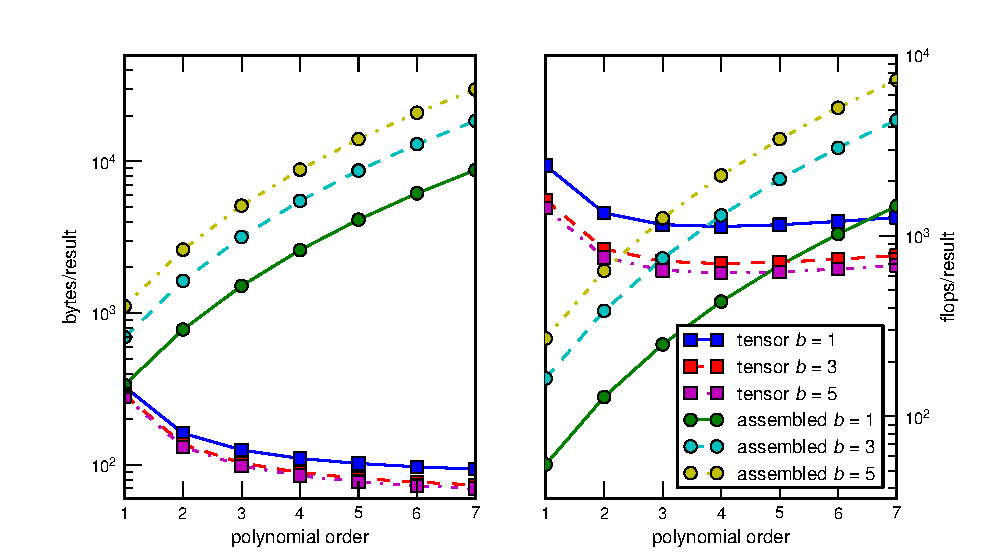
\includegraphics[width=\textwidth]{figures/TensorVsAssembly} \\
  \begin{itemize}
  \item Same linear operator, smaller to not store unassembled
  \item Use local symbolic math or AD, runtime choice of order, precondition with low-order method
  \item Dual order $h$ and $p$ FEM: \url{github.com/jedbrown/dohp}
  \item PETSc: \url{mcs.anl.gov/petsc}
  \end{itemize}
\end{frame}

\end{document}
